%%%%%%%%%%%%%%%%%%%%%%%%%%%%%%%%%%%%%%%%%
% Cover Letter Template
% Author: Cembalo Gabriele
% Personal Page: http://gcembalo.github.io
% License: MIT
%
% This template was revised by Cembalo Gabriele based on Zheng-hu Nie
% (brian.nie@gmail.com) and Fanchao Chen (chenfc@fudan.edu.cn).
% This template originates from: https://www.LaTeXTemplates.com
%
% For errors, suggestions, or improvements, please contact:
% Email: g70362643@gmail.com
%
% Version 1.1
% Last update: 2026-04-22
%
% ------------------------- Template description ---------------------------- %
%
% This is a basic academic Motivation Letter written during my MSc in
% theoretical physics seen the necessity to apply to some Summer School. This 
% template, as you can easly verify, it's inspired by Zheng-hu Nie
% and Fanchao Chen's template. You can find their template on 
% https://www.LaTeXTemplates.com .
% 
% To complete your Motivation Letter you can simply compile all the fields,
% which is pretty simple. You have just to fill your data, in the information
% section, the letter content, obviously, and the greetings.
% 
% There is no additional files, all you need is in this main file. I tried
% to comment all the code and the new command (note that the command, almost
% all of them, are from the previous template).
%
% Good work and good luck.
%

%//////////////////////////////////////////////////////////////////////////////
%                          Packages and preamble                             //
%//////////////////////////////////////////////////////////////////////////////
\documentclass[a4paper]{article}

\usepackage[
	top=1in,    % Top margin
	bottom=1in, % Bottom margin
	left=1in,   % Left margin
	right=1in,  % Right margin
	%showframe
	% Uncomment to show frames around the margins for debugging purposes
]{geometry} % Defining the geometry

\usepackage{charter} % Use the Charter font (clean serif font)
                     % the same as CV Template.
					 % (https://github.com/gCembalo/AcademicCV_Template.git)

% Defining the indentation and space between paragraphs
\setlength{\parindent}{0pt} % Paragraph indentation
\setlength{\parskip}{1em}   % Vertical space between paragraphs

\usepackage{graphicx} % Required for including images
\usepackage{fancyhdr} % Required for customizing headers and footers

% Defining the style of the page
\fancypagestyle{firstpage}{%
	\fancyhf{}                          % Clear default headers/footers
	\renewcommand{\headrulewidth}{0pt}  % No header rule
	%\renewcommand{\footrulewidth}{1pt} % Footer rule thickness
}

\fancypagestyle{subsequentpages}{%
	\fancyhf{}                          % Clear default headers/footers
	%\renewcommand{\headrulewidth}{1pt} % Header rule thickness
	%\renewcommand{\footrulewidth}{1pt} % Footer rule thickness
}

% Use the first page headers/footers style on the first page
\AtBeginDocument{\thispagestyle{firstpage}}
% Use the subsequent pages headers/footers style on subsequent pages
\pagestyle{subsequentpages}



%//////////////////////////////////////////////////////////////////////////////
%                                Document                                    //
%//////////////////////////////////////////////////////////////////////////////

\begin{document}


% -------------------------------- Header ----------------------------------- %

% If you want include the University logo to the header, with a rule under
% of it, uncomment all the command below.

%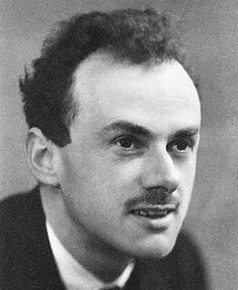
\includegraphics[width=0.35\textwidth]{logo.jpg} % Logo
%\vspace{-1em} % Pull the rule closer to the logo

%\rule{\linewidth}{1pt} % Horizontal rule

%\bigskip\bigskip % Vertical whitespace


% ------------------------------ Information -------------------------------- %

% To write, on the left, the title and the Addressee, and on the right all
% your information.

\noindent%
\begin{tabular*}{\textwidth}{@{\extracolsep{\fill}} l r @{}}
    & \today \bigskip \\ % Date on the right
    \large{\textbf{Motivation letter}} & \textbf{P.A.M. Dirac} \\
    \large{\textbf{Nobel prize for Physics}} & paul.dirac@physics.com \\
    & St. John's College, \\
    & Cambridge, London, England \\
\end{tabular*}

\bigskip % Vertical whitespace


% ---------------------------- Letter Content ------------------------------- %

% All the content of your letter.

Dear Nobel Committee for Physics,

\bigskip % Vertical whitespace

I am informed of the Royal Swedish Academy's decision. While the attention of the public is generally a source of discomfort to me, I accept this honor because the mathematical consistency of the theory demands it.

My work has been guided by the principle that physical laws should possess mathematical beauty. In seeking to unify the principles of Special Relativity with Quantum Mechanics, I found that the simplest algebraic description of the electron -- the wave equation -- required a four-component spinor.

This result was not a choice, but a necessity. The appearance of negative energy states was initially a difficulty, yet the logic of the transformation theory suggested these states could not be ignored. It led to the postulation of a "hole" in a nearly filled sea of electrons, which we now recognize as the positron.

It is my view that the fundamental laws of nature are controlled by a mathematical scheme of great elegance. If a theory is beautiful, it is more likely to be correct than an ugly one that fits experimental data. I am satisfied that the "anti-electron" has been observed, confirming that the symmetry of the equation reflects the symmetry of the world.

Nature's fundamental algebraic structures are now more visible. I have nothing further to add.

% ------------------------------- Greetings --------------------------------- %

\bigskip % Vertical whitespace

Respectfully,

\vspace{20pt} % Vertical whitespace

P.A.M. Dirac,\\
University of Cambridge. Cambridge, England.

\end{document}